%%% Local Variables:
%%% mode: latex
%%% TeX-master: t
%%% End:
\documentclass[twocolumn]{article}


% Packages
% \usepackage{fancyhdr}
\usepackage{amsmath}
\usepackage{amssymb}
\usepackage[margin=10mm]{geometry}
\usepackage{graphicx}



% Housekeeping
\pagestyle{empty}


\begin{document}
\begin{itemize}
% \item Life is fucking awesome in the United Arab Emirates!
% \item For policy makers, they care: sustainability, and the effect of
%   policies on: economy, environment and equity.
% \item \textbf{Discount Rate} Generally, you can work with constant \$ if you deal with
%   project costs. Implies minimum acceptable profitability.
% \item \textbf{Raising Capital} Debt (borrowing) Equity (selling parts
%   of the company)
% \item \textbf{WACC} Can be used as a metric, a reasonable
%   approximation of DR; But it does neither account for project risk
%   nor opportunity cost.
% \item \textbf{Internal Rate of Return} Discount rate for which NPV is
%   $0$. In the context of savings and loans the IRR is also called the
%   effective interest rate. Because the internal rate of return is a
%   rate quantity, it is an indicator of the efficiency, quality, or
%   yield of an investment. This is in contrast with the net present
%   value, which is an indicator of the value or magnitude of an
%   investment. 
% \item \textbf{LCOE} Levelized Energy Cost is the price at which
%   electricity must be generated from a specific source to \textbf{break even}
%   over the lifetime of the project. It is an economic assessment of
%   the cost of the energy-generating system including all the costs
%   over its lifetime: initial investment, operations and maintenance,
%   cost of fuel, cost of capital, and is very useful in calculating the
%   costs of generation from different sources.
% \item Issues with LCOE: However, care should be taken in comparing
%   different LCOE studies and the sources of the information as the
%   LCOE for a given energy source is \textbf{highly dependent} on the
%   assumptions, financing terms and technological deployment analyzed.
% \item \textbf{Break Even} is the point at which total cost and total
%   revenue are equal.
% \item \textbf{Net Present Value} In finance, the net present value
%   (NPV) of a time series of cash flows, both incoming and outgoing, is
%   defined as the sum of the present values (PVs) of the individual
%   cash flows of the same entity. NPV can be described as the
%   “difference amount” between the sums of discounted: cash inflows and
%   cash outflows. It compares the present value of money today to the
%   present value of money in the future, taking inflation and returns
%   into account. 
% \item Yet some more notes on NPV.
%   \begin{itemize}
%   \item The investment horizon of all possible investment projects
%     considered are equally acceptable to the investor.
%   \item The 10\% discount rate is the appropriate (and stable) rate to
%     discount the expected cash flows from each project being
%     considered. Each project is assumed equally speculative. 
%   \item the shareholders can't get above a 10\% return on their money
%     if they were to directly assume an equivalent level of risk.  
%   \end{itemize}
% % \item Life is fucking awesome in the United Arab Emirates!
\item \textbf{Dual Carbon Constraints} Fossil fuels are finite and
  burning them contributes to climate change and pollution.
\item \textbf{Conservation of Energy} During an interaction, energy
  can change from one form to another but the total amount of energy
  remains constant.  
\item \textbf{Second Law of Thermaldynamics} It asserts that energy
  has quality as well as quantity, and actual processes occur in the
  direction of decreasing quality of energy.
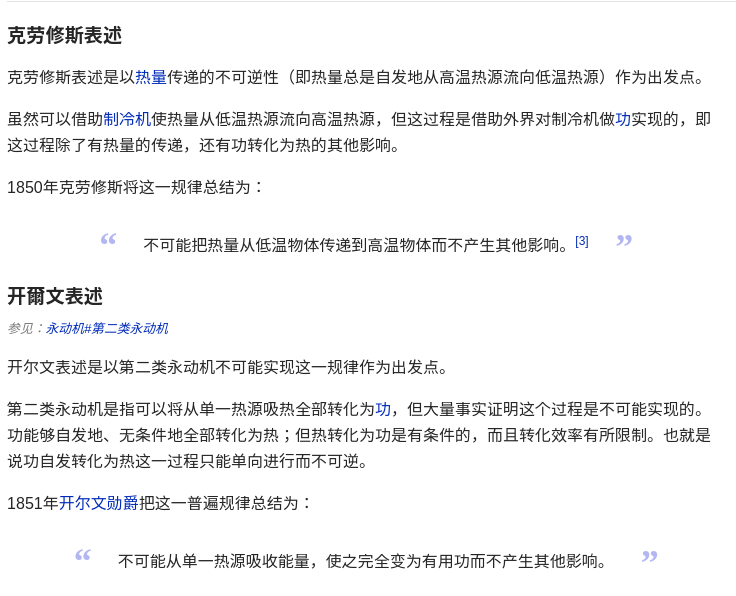
\includegraphics[scale=0.45]{snapshot102}
\par
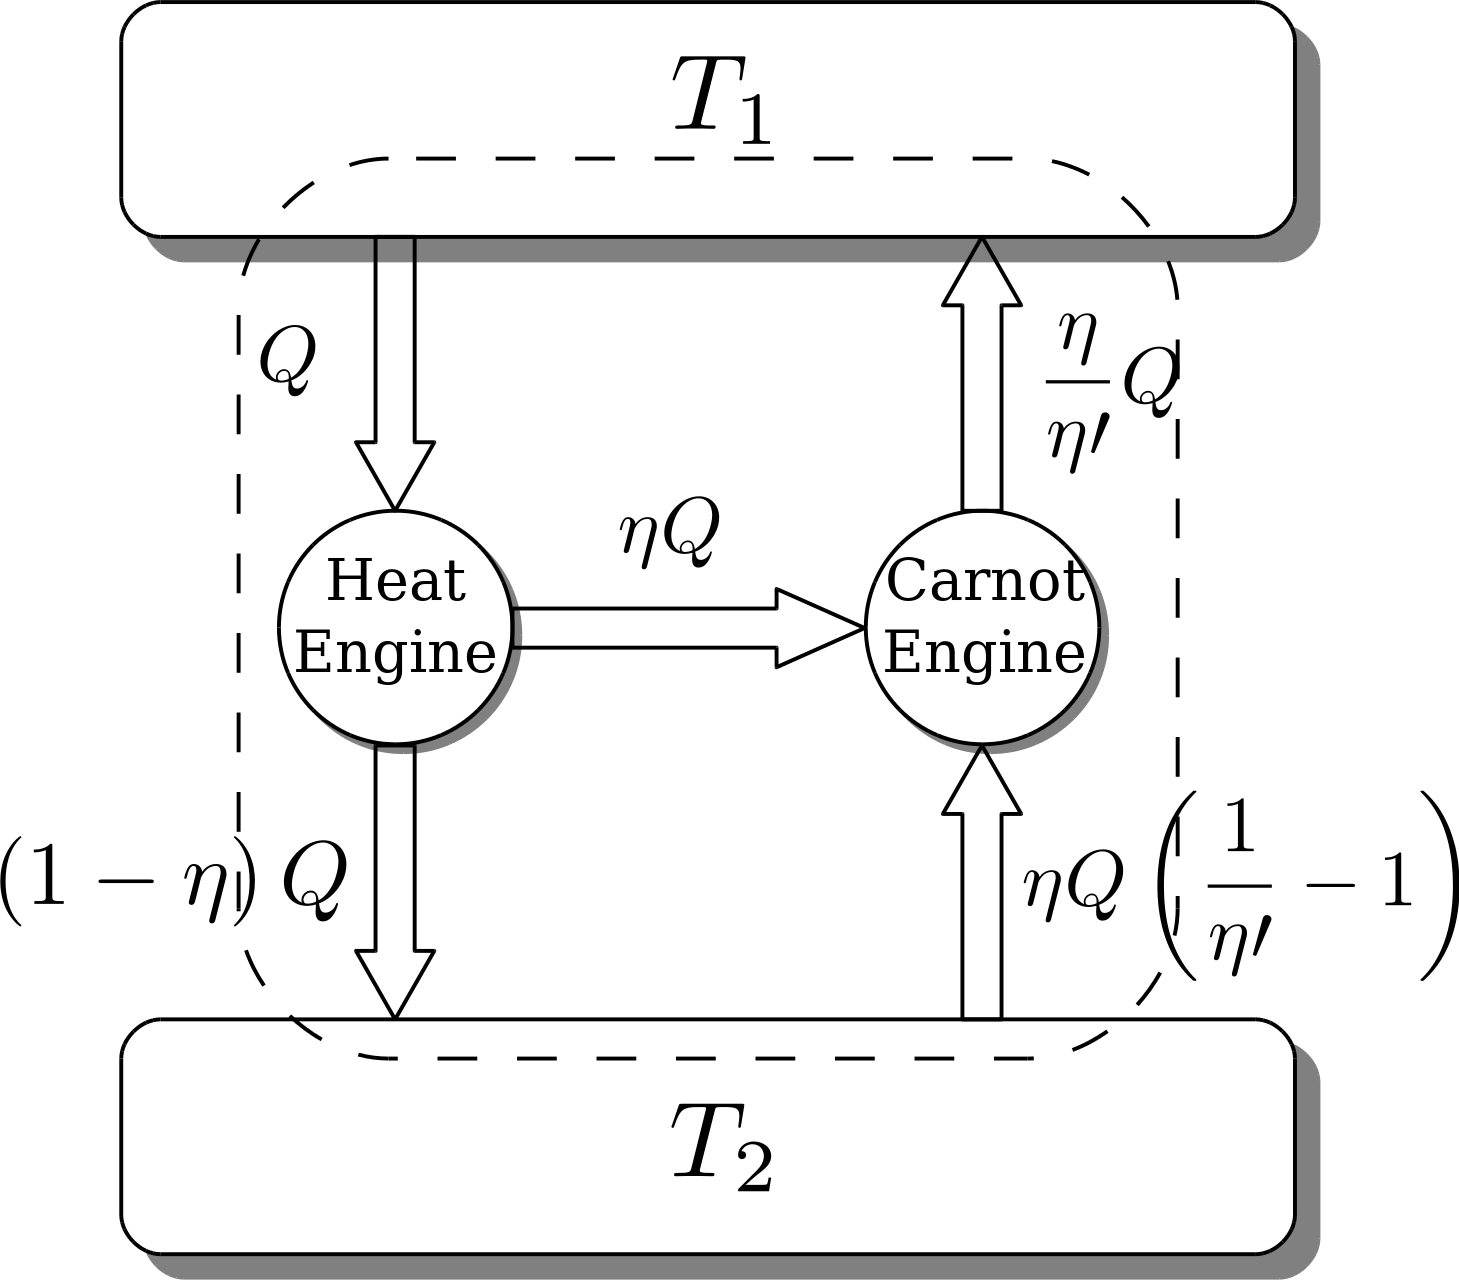
\includegraphics[scale=0.16]{Carnot}
\par
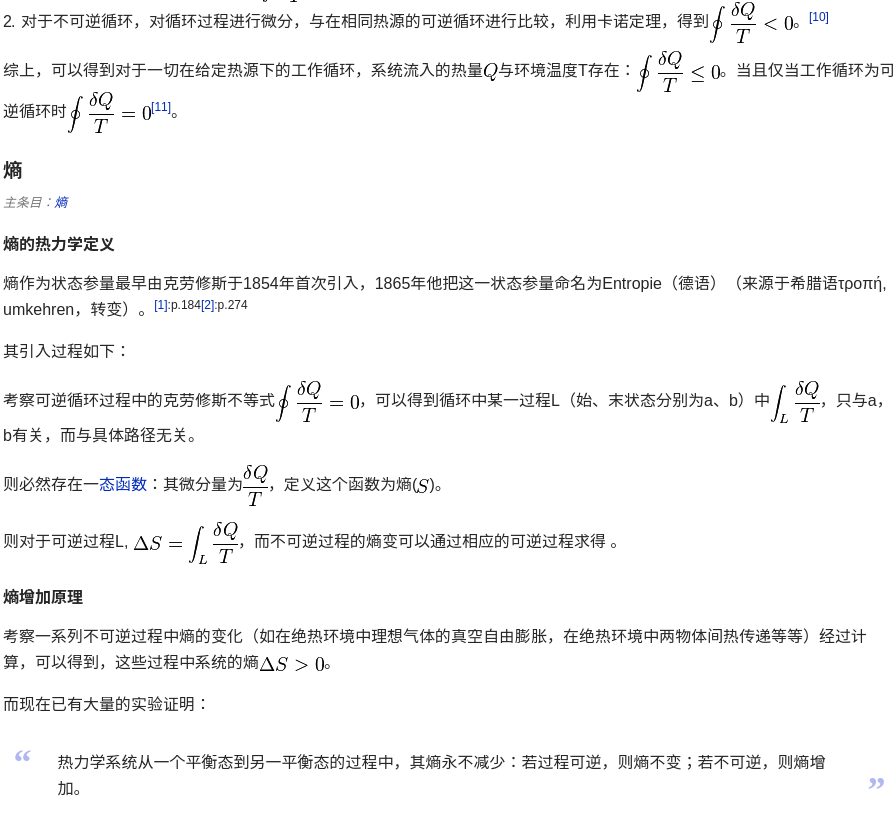
\includegraphics[scale=0.32]{snapshot103}
\item Thermodynamics deals only with the \textbf{change} of the total
  energy. 
\item \textbf{First Law of Thermodynamics} The law of conservation of
  energy states that the total energy of an isolated system is
  constant; energy can be transformed from one form to another, but
  cannot be created or destroyed. $Q-W=\Delta U$. Or in another form,
  $Q=\Delta U+W$.
\item \textbf{Thermal Efficiency} Net work output $\div$ Total Heat
  Input.
\item \textbf{Enthalpy} is defined thermodynamic potential, designated
  by the letter "H", that consists of the internal energy of the
  system (U) plus the product of pressure (p) and volume (V) of the
  system. $H=U+pV$ and when the pressure is assumed constant, we have
  $\delta H=\delta U+p\delta V$.
\item \textbf{WACC} is just a fancy name for Weighted Average Cost of
  Capital. 
\item \textbf{LCOE} Levelized Energy Cost is the price at which
  electricity must be generated from a specific source to break even
  over the lifetime of the project.
\item \textbf{Biomass} Renewable; Connected to farming and
  agriculture; Multiuse; Environmental concerns include land and water
  use, fertilizer and other nutrient requirements; Naturally diffuse
  and distributed. 
\item \textbf{Sustainable Bioenergy} The use of water, land and the
  debate between food and fuel.
\item \textbf{Hydrothermal} Two main types, dry steam
  (vapor-dominated) reservoirs and hot water (liquid-dominated).
\item \textbf{Geothermal Challenges} Characterizing and Predicting;
  Accessing; Engineering; Sustaining; Monitoring.
\item \textbf{Solar Technologies} Non-Concentrated, Photovoltaic,
  Solar Thermal; Concentrated, Concentrated Photovoltaic, Concentrated
  Solar Power. 
\item \textbf{PV and CSP} Solar photovoltaic (PV) directly converts
  solar energy into electricity using a PV cell made of a
  semiconductor material. Concentrating solar power (CSP) devices
  concentrate energy from the sun’s rays to heat a receiver to high
  temperatures. This heat is transformed first into mechanical energy
  (by turbines or other engines) and then into electricity – solar
  thermal electricity (STE).
\item \textbf{CSP Technologies} Parabolic trough, Linear Fresnel
  Reflector, Power tower and Parabolic Dish/Stirling. 
% \item \textbf{CSP Storage Techniques} Active storage: direct system,
%   indirect system. Two tank, single tank. To be more specific: Molten
%   salt, volumetric air receiver, direct steam
  generation. \emph{Physical and Chemical} process. Sensible heat,
  latent heat; Chemical Energy.
\item \textbf{Thermal Storage} Tested technologies: single tank oil
  thermocline with filler materials, Two-tank Oil
  Technology. Commercial:  Two-tank Molten Salt, Saturated Steam.
  Under development: High-temperature Concrete Regenerator Type
  Storage, Combined sensible \& Latent heat, Cascade Latent Heat
  Storage. Under research: Fluidized Bed Sand Storage, Conventional
  Heat Transfer Fluid, Formulate New Molten salts Compositions.
\item \textbf{Nuclear Sustainability} On the other hand, NPPs are cheap to operate: the existing
operating NPPs, for which the initial capital investments
are largely depreciated, are among the lowest cost
generators. Not surprisingly, interest has grown in
extending NPP operating lifetimes from their initial
licensed lifetimes of 30–40 years, and actual license
extensions of up to 60 years are already a reality. 
\item Nuclear energy comes from uranium, a nonrenewable resource that
  must be mined. 
\item 13 percent of the world’s electricity comes from nuclear power
  plants that emit little to no greenhouse gases. Nuclear power
  facilities can produce energy at a 91 percent efficiency rate 24/7,
  while maintaining the method with the lowest emissions. More than 70
  percent of America’s emission-free power comes from nuclear energy
  sources. 
\item The building of new nuclear facilities creates between 1,400 and
  3,500 jobs for construction workers, and after the facility is built
  maintains 400 to 700 permanent positions paying roughly 36 to 44
  percent more than the average salary of the surrounding
  area. American nuclear energy facilities are the highest regulated
  plants in the world, subject to more scrutinous observations and
  regulations. 
\item The average exposure for each worker in the U.S. nuclear energy industry is 290
mrem, which is only one-third of the 900 mrem per year occupational exposure of
airline pilots and cabin crews who regularly fly the high-altitude New York -Tokyo
route.
\item Recent increases in international fossil fuel market prices
have eliminated the margins for natural gas and coal,
leaving nuclear power as the least-cost electricity
generation option for base-load electricity generation.
\item Moreover, in most countries, the cost of containing,
storing, and disposing of nuclear waste is included in the
price of the electricity generated.
\item Significant health impacts from NPPs thus arise only from
major accidents that release radiation. Caused by
serious design flaws coupled with major operator errors.
\item \textbf{Probability of Occurrence} over $N$ number of years:
  $P=1-{(1-p)}^{n}$.
\item \textbf{Gringorten Formula} $T=\frac{n+0.12}{i-0.44}$
\item To find the power generated (in Watts) by a wind turbine:
  $P=\frac{1}{2}\rho Av^{3}C_{p}$ air density, swept area, wind speed
  and  the power coefficient.
\item Nuclear power
 can be a cost-effective electricity supply technology,
especially at current fossil fuel price levels;
 surpasses other options in internalizing its
externalities;
 is a cost-effective way to reduce carbon emissions
from an electricity generation (any internalization
of greenhouse gas emissions further improves its
competitively);
 manages its waste safely;
 has an incomparable industrial safety record with a
philosophy of continual improvement; and
 is not a principal contributor to proliferation risks,
and that halting or reversing the expansion of
nuclear power would not appreciably reduce such
a risk.
\item Vertical wind speed power law profile:
  $v_{2}=v_{1}*(\frac{z_{2}}{z_{1}})^{\alpha}$.




\end{itemize}
\end{document}


